\ylDisplay{Lambid} % Ülesande nimi
{Mihkel Kree} % Autor
{lahtine} % Voor
{2013} % Aasta
{G 9} % Ülesande nr.
{7} % Raskustase
{
% Teema: Elektriahelad
\ifStatement
Juku ehitas kodus niisuguse elektriskeemi nagu joonisel näidatud, kasutades
selleks kuut ühesugust takistit takistusega $R=\SI{10}{\ohm}$, nelja
ühesugust lampi takistusega $r=\SI{20}{\ohm}$ ning pingeallikat
elektromotoorjõuga
$\mathcal{E}=\SI{5}{\volt}$. Arvutage igas lambis (joonisel tähised 1, 2, 3,
4) eralduv võimsus. Pingeallika sisetakistusega mitte arvestada.
\begin{center}
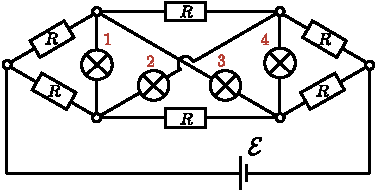
\includegraphics[width=0.6\linewidth]{2013-lahg-09-lambidJoonis-crop}
\end{center}
\fi


\ifHint
Paneme tähele, et sümmeetria tõttu on lampide 1 ja 4 otspunktide potentsiaalid võrdsed.
\fi


\ifSolution
Paneme tähele, et skeemi sümmeetria tõttu ei läbi vool lampi 1, sest selle otstel on võrdsed potentsiaalid. Sama kehtib lambi 4 kohta. Joonistame skeemi ümber, ühendades lambi 1 otspunktid omavahel kokku, sama teeme ka lambi 4 otspunktidega. Saame võrdlemisi lihtsa skeemi, mis koosneb kolmest jadamisi ühendatud paralleelühendusest, nagu joonisel näidatud. 

\begin{center}
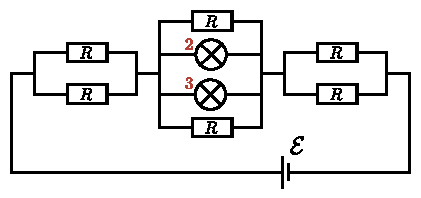
\includegraphics[width=0.8\textwidth]{2013-lahg-09-ahelLah.pdf}
\end{center}

Arvutame ahela kogutakistuse
\[R_t = \frac{R}{2} + \frac{1}{\frac{1}{R}+\frac{1}{r}+\frac{1}{r}+\frac{1}{R}}+\frac{R}{2} =\frac{4}{3}R,\]
kus arvestasime, et $r=2R$, kusjuures keskmise paralleelühenduse takistuseks tuli $R_k=R/3$, mis moodustab $1/4$ osa kogutakistusest, seega langeb keskmisele osale ka $1/4$ osa patarei pingest ehk $V_k = \mathcal{E}/4 = \SI{5/4}{V}$. Nüüd on juba lihtne avaldada lampides 2 ja 3 eralduv võimsus
\[P_2=P_3=\frac{V_k^2}{r}=\frac{25}{16\cdot 20}\SI{}{W}\approx\SI{0,08}{W}.\]
Lampides 1 ja 4 mõistagi võimsust ei eraldu.
\fi


\ifEngStatement
% Problem name: Lamps
Juku built a circuit diagram that is shown in the figure using six identical resistors of resistance $R=\SI{10}{\ohm}$, four identical lamps of resistance $r=\SI{20}{\ohm}$ and a voltage source with an electromotive force $\mathcal{E}=\SI{5}{\volt}$. Calculate the power dissipated by each lamp (in the figure marked as 1, 2, 3, 4). Do not account for internal resistance of the voltage source.
\begin{center}
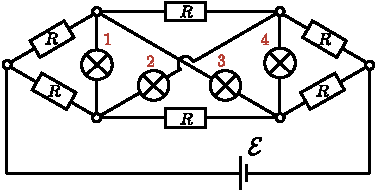
\includegraphics[width=0.6\linewidth]{2013-lahg-09-lambidJoonis-crop}
\end{center}
\fi


\ifEngHint
Let us notice that due to the symmetry the potentials of the terminals of the lamps 1 and 4 are equal.
\fi


\ifEngSolution
We notice that due to the diagram’s symmetry no current goes through the lamp 1 because there are equal potentials on its leads. The same applies to the lamp 4. Let us redraw the diagram by connecting the leads of the lamp 1 with each other, we do the same with the leads of the lamp 4. We get a relatively simple diagram that consists of three parallel connections which are connected in series, as shown in the figure.
\begin{center}
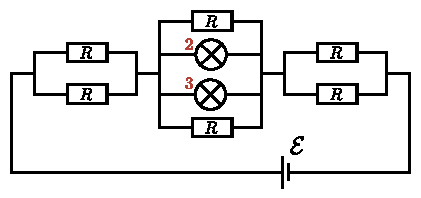
\includegraphics[width=0.8\textwidth]{2013-lahg-09-ahelLah}
\end{center}
We calculate the total resistance of the diagram
\[R_t = \frac{R}{2} + \frac{1}{\frac{1}{R}+\frac{1}{r}+\frac{1}{r}+\frac{1}{R}}+\frac{R}{2} =\frac{4}{3}R,\] 
where we took into account that $r=2R$, moreover the resistance of the middle parallel connection was $R_k=R/3$ which is $1/4$ of the total resistance. Therefore $1/4$ of the battery’s voltage is applied to the middle part meaning $V_k = \mathcal{E}/4 = \SI{5/4}{V}$. Now it is easy to express the power dissipated by the lamps 2 and 3
\[P_2=P_3=\frac{V_k^2}{r}=\frac{25}{16\cdot 20}\SI{}{W}\approx\SI{0,08}{W}.\] 
Naturally no power dissipates in the lamps 1 and 4.
\fi
}